%*************************************************************
\chapter{CSCW \& Groupware}\label{ch:CSCWDesign} \index{CSCW}
%*************************************************************

	Der Begriff >>Computer Supported Cooperative Work<< (\ac{CSCW}) bezeichnet ein multidisziplinäres Forschungsgebiet, das die kooperative Zusammenarbeit mehrerer Gruppen untersucht und Technologien zu ihrer Unterstützung entwickelt. \ac{CSCW} existiert seit den frühen achtziger Jahren. Um herauszufinden, wie die Technik Menschen bei ihrer Zusammenarbeit unterstützen kann, organisierten Irene Greif und Paul Cashman im Jahre 1984 einen Workshop für Personen, die sich mit der Arbeitsweise von Menschen auseinandersetzten \citep{Grudin:1994}. Unter diesen Personen befanden sich Spezialisten aus verschiedenen wissenschaftlichen Bereichen, wie zum Beispiel Ökonomie, Sozialpsychologie, Anthropologie, Ethnologie und Pädagogik. Dieser Workshop war der Versuch der Techniker, Teamarbeit besser zu verstehen und folglich unterstützende Technologien entwickeln zu können \citep{Grudin:1994, Rama:2006p245}. Seither hat \ac{CSCW} sich zu einem nahezu riesigen wissenschaftlichen Forschungsgebiet entwickelt, dem sich heute unzählige Experten widmen. Trotzdem sind sich die Wissenschaftler nicht immer ganz einig bei der Definition des Begriffes \ac{CSCW}. Die Bedeutung von >>Cooperative Work<< erscheint nicht eindeutig und führt häufig zu unterschiedlichen Interpretation seitens wissenschaftlicher Autoren \citep{Gerlicher:2007p241}. Einige setzen >>Cooperation<< gleich mit >>Collaboration<<, andere hingegen unterscheiden die beiden Begriffe sehr strikt. Dillenbourg et al. definieren die Begriffe beispielsweise so: 
	
	\medskip\begin{quote}{>>Cooperation and collaboration do not differ in terms of whether or not the task is distributed, but by virtue of the way in which it is divided; in cooperation the task is split (hierarchically) into independent subtasks; in collaboration cognitive processes may be (heterarchically) divided into intertwined layers. In cooperation, coordination is only required when assembling partial results, while collaboration is “...„ a coordinated, synchronous activity that is the result of a continued attempt to construct and maintain a shared conception of a problem.<<} \begin{flushright}\citep{Dillenbourg:1995} \end{flushright}\end{quote}
	
	\medskip Die beiden Begriffe unterscheiden sich also nicht darin, \emph{ob} Arbeit auf mehrere Individuen aufgeteilt wird oder nicht, sondern in der Art und Weise, \emph{wie} sie aufgeteilt wird. Bei >>Cooperation<< wird die Arbeit in einzelne, unabhängige Module aufgeteilt, die zuerst abgewickelt und danach wieder zu einem Ganzen zusammengesetzt werden können. Koordination wird in diesem Fall hauptsächlich beim Zusammenfügen der Module benötigt. >>Collaboration<< hingegen ist eine koordinierte, synchrone Aktivität und resultiert aus dem fortwährenden Versuch, eine gemeinsame Auffassung eines Problems zu konstruieren und zu erhalten.
	
	In dieser Arbeit werden die beiden Begriffe synonym verwendet, da sich beide aus dem Englischen als >>Zusammenarbeit<< übersetzen lassen. Um den Begriff \ac{CSCW} jedoch besser zu verstehen, sollen weitere Definitionen von >>Cooperative Work<< begutachtet werden.
	
	Die Ökonomie kennt den Begriff >>Cooperative Work<< schon sehr lange und Marx definiert ihn als mehrere Individuen, die gemeinsam in einer koordinierten Art und Weise an einem oder mehreren, zusammengehörigen Produktionsprozessen arbeiten \citep{Marx:1867}. Im deutschen Sprachraum wurde diese Definition im 19. Jahrhundert häufig durch andere Autoren wiederverwendet, jedoch gibt es sehr viele Formen von >>Cooperative Work<< und es gibt in der Literatur keine klare Trennung zwischen Begriffen wie >>Cooperative Work<<, >>Collaborative Work<<, >>Collective Work<< und >>Group Work<< \citep{Bannon:1990p244}.
	
	Die Definition von >>Cooperative Work<< nach Bannon und Schmidt besagt, dass sie im Allgemeinen aus Arbeitsprozessen besteht, die ein Produkt oder ein Service hervorbringen. Ein typisches Merkmal dieser Arbeitsform ist die Planung der Abwicklung, die vor Beginn der eigentlichen Arbeit durchgeführt wird. >>Cooperative Work<< beinhaltet \emph{direkte}, \emph{indirekte}, \emph{verteilte} und \emph{kollektive} Arten der Interaktion. \emph{Kollektiv} in einer Gruppe geleistete Arbeit, sprich >>Group Work<< ist lediglich eine spezielle Form von >>Cooperative Work<<. Es ist aber ebenfalls möglich, dass >>Cooperative Work<< von einer geographisch \emph{verteilten} Gruppe halb autonomer Personen geleistet wird, die bei der Abwicklung strategisch nach eigenem Ermessen vorgehen. Zusätzlich kann >>Cooperative Work<< \emph{indirekt}, über den Arbeitsprozess selbst, als auch \emph{direkt}, durch Kommunikation zwischen den einzelnen Gruppenmitgliedern durchgeführt werden. \citep{Bannon:1990p244}
	
	\bigskip Die Erkenntnisse, die bei der Erforschung von \ac{CSCW} gewonnen werden, verwendet man dazu, sinnvolle Groupware \index{Groupware} zu konzipieren. Groupware bezeichnet also die technische und praktische Umsetzung, die auf den Theorien der \ac{CSCW}-Forschung basiert. Alle Systeme, Applikationen und Werkzeuge, die \ac{CSCW} unterstützen, können somit unter dem Begriff Groupware zusammengefasst werden \citep{Koch2008, Gerlicher:2007p241}. Häufig werden diese Systeme auch als >>kollaborative Software<< bezeichnet \citep{Bannon:1990p244}. Gerlicher und Ansgar definieren Groupware wie folgt:
	
	\medskip\begin{quote}>>Der Begriff Groupware bezeichnet ein aus Software und eventuell spezifischer Hardware bestehendes System, das die Zusammenarbeit im Team durch die Schaffung von Kommunikations- und/oder Koordinationslösungen unterstützt oder ermöglicht.<< \begin{flushright}\citep{Gerlicher:2007p241}\end{flushright}\end{quote}
	
	\medskip Michael Koch definiert Groupware als:
	
	\medskip\begin{quote}>>[...] Nevertheless, there are some technologies and tools [Groupware] that facilitate shaping [...] socio-technical systems. For these technologies and tools the term Groupware is used. In contrast to traditional computer systems that are primarily designed for a single user, the major goal of Groupware is to assist a group of users in communicating, in collaborating, and in coordinating their activities.<< \begin{flushright}\citep{Koch2008}\end{flushright}\end{quote}
	
	\medskip Groupware unterscheidet sich also von >>Ein-Benutzer-Systemen<< darin, dass sie für mehrere Benutzer konzipiert ist und versucht, die höchste Effizienz und Flexibilität für die Teamarbeit dieser Benutzer zu gewährleisten. In dieser Hinsicht hat Groupware einige Vorteile gegenüber single-user Software. Gerlicher und Ansgar nennen die folgenden Gründe, warum Groupware eingesetzt wird: 
	
	\begin{itemize}
		\item {Verbesserung der Kommunikation in der Gruppe}
		\item {Ermöglichen von Kommunikation, wo sie sonst nicht möglich wäre}
		\item {Ermöglichen von Telearbeit (für geographisch entfernte Benutzer)}
		\item {Einsparung von Reisekosten}
		\item {Bündelung von Fachwissen und Gedankenaustausch in der Gruppe}
		\item {Bildung von Gruppen mit gemeinschaftlichem Interesse}
		\item {Reduktion von zeitlichem und finanziellen Aufwand bei der Koordination von Gruppen}
		\item {Problemlösung in der Gruppe}
		\item {Erlangung neuer Kommunikationsmöglichkeiten, beispielsweise dem anonymen oder strukturierten Informationsaustausch}
	\end{itemize}
	\begin{flushright}
		\citep{Gerlicher:2007p241}
	\end{flushright}
	
	Demgegenüber steht die Schwierigkeit, erfolgreiche Groupware Systeme zu entwickeln. Im Gegensatz zu single-user Software ist dies äußerst komplex und es gibt viele kritische Faktoren. Zum einen sind die technischen Voraussetzungen diffiziler, weitaus entscheidender ist jedoch, dass Groupware von der Gruppe lebt und daher ist die Akzeptanz durch die Zielgruppe maßgebend für den Erfolg von Groupware \citep{Gerlicher:2007p241}.
	
	\medskip \ac{CSCW} soll aber nicht nur Technologien und Werkzeuge zur Unterstützung von Kollaboration bereitstellen, sondern auch soziotechnische Systeme entwickeln \citep{Koch2008}. In den 1950er Jahren wurden Experimente durchgeführt, bei denen technische Systeme in mehrere verschiedene soziale Gruppen eingeführt wurden. Dabei stellte man fest, dass die Technologieeinführung in den Gruppen sehr unterschiedliche Auswirkungen hatte. Dadurch kamen die Wissenschaftler zum Schluss, dass das technische, als auch das soziale System auf diese Zusammenführung hin optimiert werden müssen, um ein erfolgreich funktionierendes, einheitliches Gesamtsystem hervorzubringen \citep{Koch2008}. Wenn diese Optimierung nicht passiert und bei der Einführung der Technik die sozialen Aspekte und Eigenheiten nicht berücksichtigt werden, kann das Ergebnis nur suboptimal sein. Soziale Prozesse sind die Basis für die Entwicklung und das Design von neuen Technologien und Systemen und umgekehrt strukturieren diese Technologien die Möglichkeiten des sozialen Austauschs. Für den Erfolg von neuen Technologien ist es unerlässlich, diese sozialen und technischen Aspekte bei Entwicklung und Design mit einzubeziehen \citep{Mumford:2000}.
	
	Das Forschungsgebiet \ac{CSCW} versucht also soziale Interaktion in Gruppen und Teams zu verstehen und technische Systeme zur Unterstützung selbiger zu konzipieren, zu entwickeln und zu evaluieren \citep{Koch2008}.

\section{Klassifikation von CSCW} \index{CSCW!Klassifikation}

\ac{CSCW} kennt zwei Dimensionen: Raum und Zeit. Dies sind die Kriterien, nach denen \ac{CSCW} und Groupware eingeteilt werden. \autoref{fig:ramaCSCW} illustriert die Kategorisierung von \ac{CSCW} und ordnet den vier sich aus der Überschneidung der Dimensionen ergebenden, Quadranten einige Beispiele zu. 

Der erste Quadrant umfasst alle Systeme und Technologien, bei denen die Benutzer zur selben Zeit am selben Ort sein müssen. Beispielsweise könnten sich zwei Personen in einem Meetingraum treffen und gemeinsam Konzepte an einem digitalen Whiteboard ausarbeiten. Sie teilen zeitliche und räumliche Komponenten miteinander. 

\begin{figure}
	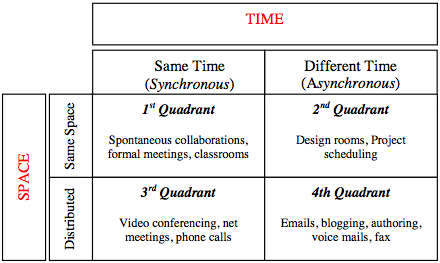
\includegraphics[width=\textwidth]{gfx/ramaCSCWQuadranten.png}
	\caption[CSCW-Kategorien \newline \citep{Rama:2006p245}]{Die Grafik illustriert die Unterteilung von CSCW in vier Kategorien, die sich durch ihre räumlichen und zeitlichen Eigenschaften unterscheiden. Der Faktor Zeit definiert, ob Zusammenarbeit in einer Gruppe synchron oder asynchron passiert und der Faktor Raum definiert, ob sie am selben oder an geographisch distanzierten Orten stattfindet.}
	\label{fig:ramaCSCW}
\end{figure}

Der zweite Quadrant kategorisiert all jene Technologien, die Personen am selben Ort zu unterschiedlichen Zeiten nutzen können. Ein Designraum mit elektronischen Geräten könnte ein Beispiel dafür sein. Angenommen, eine Person überlegt sich ein Konzept und zeichnet Skizzen auf ein Tabletop Display. Zu einem späteren Zeitpunkt, als die Person den Raum bereits verlassen hat, kommt eine andere Person herein, arbeitet mit den Skizzen weiter und entwickelt eigene Konzepte, die sie wiederum auf dem Tabletop festhält. 

Zum dritten Quadranten gehören alle Systeme, die zur selben Zeit an verschiedenen Orten eingesetzt werden können. Das wohl bekannteste dieser Systeme ist das Telefon. Es kann nur von zwei Personen gleichzeitig benutzt werden, aber die Personen können sich dazu an beliebigen Orten befinden.

Im vierten Quadranten befinden sich alle Technologien, die zu unterschiedlichen Zeiten an unterschiedlichen Orten zum Einsatz kommen. E-Mail, das elektronische Nachrichtensystem, ist ein gutes Beispiel solcher Groupware. Um auf diesem Wege zu kommunizieren, müssen zwei Personen weder gleichzeitig damit interagieren, noch sich am selben Ort befinden. 

\medskip Gerlicher definiert zusätzlich eine weitere Kategorie in \ac{CSCW}, auf die im Abschnitt \nameref{sec:multisynchronousCSCW} näher eingegangen werden soll, nachdem die vier grundlegenden Kategorien im folgenden näher definiert werden.

\subsection{Asynchrone Systeme} \index{CSCW!Asynchrone Systeme}

Unter asynchroner Groupware versteht man Systeme, die keine Echtzeitanforderungen erfüllen müssen. Das bedeutet, dass die Nutzung dieser Systeme im Normalfall zeitversetzt erfolgt. Die wohl bekannteste asynchrone Groupware-Anwendung ist die digitale Übermittlung von Textnachrichten in Form einer \emph{E-Mail}. Diese Nachrichten können an und von mehreren Personen versendet, empfangen und weitergeleitet werden. Dabei müssen Absender und Empfänger nicht gleichzeitig online sein, denn die \emph{E-Mail} kann zu jedem beliebigen Zeitpunkt vom Empfänger abgerufen werden.

Eine andere, jedoch der \emph{E-Mail} sehr ähnliche Form asynchroner Groupware, sind \emph{Newsgroups und Mailinglisten} \citep{Gerlicher:2007p241}. Sie dienen dem Nachrichtenaustausch in einer größeren Gruppe an Benutzern. \emph{Newsgroups} zeigen Nachrichten nur dann an, wenn ein Benutzer diese direkt anfordert, \emph{Mailinglisten} hingegen werden automatisch an all jene Personen weitergeleitet, welche die entsprechende Liste abonniert haben.

Auch \emph{Workflow-Management-Systeme} werden von Gerlicher und Ansgar \citep{Gerlicher:2007p241} zur asynchronen Groupware gezählt, da sie die Arbeit unterschiedlicher Personen in einer Organisation regeln. Sie dienen der Steuerung arbeitsteiliger Prozesse. Man bezeichnet sie auch als \emph{Geschäftsprozess-Management-Systeme}.

Das World Wide Web (WWW) ist ein \emph{Hypertext-basiertes System} und gehört ebenfalls zur asynchronen Groupware \citep{Gerlicher:2007p241}, da es einer sehr großen Anzahl an Personen ermöglicht, auf digitalem Wege Informationen auszutauschen. \emph{Hypertext-basierte Systeme} nutzen das Internet oder ein bestimmtes Intranet, um ihre Dienste über einen Webbrowser zugänglich zu machen. Solch eine Webschnittstelle kann prinzipiell für fast jede Art der asynchronen Groupware implementiert werden. 

Schlussendlich nennen Gerlicher und Ansgar noch \emph{Gruppenkalender} als asynchrones Groupware System. Der \emph{Gruppenkalender} ist ein Tool, das sehr häufig in größeren Unternehmen eingesetzt wird. Er ermöglicht die Terminplanung und Koordination von vielen Personen. Terminkonflikte werden automatisch erkannt und das System kann eigenständig jene Zeiträume finden, zu denen jeder erforderliche Teilnehmer eines Meetings frei zur Verfügung steht. Dies setzt jedoch eine gute Datenpflege aller Benutzer voraus und wird teilweise als unangenehmer Eingriff in die Privatsphäre empfunden \citep{Gerlicher:2007p241}.
\clearpage

\subsection{Synchrone Systeme} \index{CSCW!Synchrone Systeme}

Dem gegenüber stehen synchrone Groupware Systeme, die sich dadurch charakterisieren, dass Benutzer zeitgleich auf Daten und Informationen zugreifen \citep{Gerlicher:2007p241}. Ein Beispiel dafür sind \emph{elektronische Tafeln}, denn sie erlauben mehreren Nutzern, die sich an unterschiedlichen Orten befinden, auf eine für alle sichtbare Fläche zu zeichnen. Häufig werden solche Tafeln bei Besprechungen eingesetzt, bei denen die Teilnehmer nicht im selben Raum sind. Dadurch wird es möglich, Konzepte und Ideen besser zu kommunizieren und für die anderen greifbarer zu machen.

\emph{Application Sharing Systeme} zählen ebenfalls zur synchronen Groupware und gestatten das Teilen von Drittapplikationen mit anderen Personen \citep{Gerlicher:2007p241}. Man bezeichnet diese Anwendungen im Englischen auch als \emph{Remote Desktop}\footnote{Zu Deutsch: Entfernter Schreibtisch. Gemeint ist damit die virtuelle Schreibtischfläche des Betriebssystems.}. Dadurch wird es möglich, mit geografisch distanzierten Kollegen an jedem beliebigen Programm zu kooperieren. Beide Benutzer sehen die Applikation, die auf einem der Computer läuft und können mit ihr interagieren. 

Weitere synchrone Systeme sind \emph{Video- und Multimediale Konferenzsysteme} \citep{Gerlicher:2007p241}. Erstere übertragen Video und Audio an mehrere verteilte Computer und werden eingesetzt, um virtuelle Meetings abzuhalten. Die Teilnehmer befinden sich meist an verschiedenen Orten und können so fast genauso kommunizieren, als würden sie sich in einem Raum befinden. Letztere bieten zusätzlich die Möglichkeit, multimediale Inhalte (beispielsweise Präsentationen) an die Teilnehmer der Konferenz zu übertragen. Systeme zu Entscheidungsfindung sind oft ein integraler Bestandteil solcher Software und bieten Werkzeuge für Ideenfindung und Brainstorming. Über auf diesem Wege generierte Konzepte kann dann abgestimmt und so die Spreu vom Weizen getrennt werden. 

\emph{Chat-Systeme}, ebenfalls der synchronen Groupware zuzuordnen, sind weitgehend bekannt und werden sehr häufig eingesetzt. Benutzer können durch diese Anwendungen in Echtzeit untereinander Textnachrichten austauschen und so eine Konversation führen, als säßen sie sich gegenüber. 

\subsection{Multisynchrone Systeme}\label{sec:multisynchronousCSCW}\index{CSCW!Multisync. Systeme}

\emph{Versionsverwaltungssysteme} werden von Gerlicher und Ansgar als multisynchrone Systeme definiert \citep{Gerlicher:2007p241}. Häufig werden diese in Softwareprojekten und auch bei der Erstellung von umfangreichen Dokumenten, beispielsweise Büchern eingesetzt. Das System übernimmt die Verwaltung der Dateien und sichert die Konsistenz der Daten. Es wird dadurch möglich, dass mehrere Personen gleichzeitig an der selben Datei arbeiten. Tatsächlich haben aber alle Benutzer eine eigene Kopie der Datei und das System synchronisiert die Dateien im Nachhinein selbständig. Ein weiterer großer Vorteil von \emph{Versionsverwaltungssystemen} ist die Nachvollziehbarkeit von Änderungen \citep{Gerlicher:2007p241} an einzelnen Dateien. Das System legt für jede neue Version einer Datei ein Backup ab, das zu einem späteren Zeitpunkt bei Bedarf wiederhergestellt werden kann. Es ist zu jedem Zeitpunkt klar, wer welche Änderungen an einer bestimmten Datei durchgeführt hat. 

\bigskip Es wird deutlich, dass \ac{CSCW} und Groupware sehr weitläufig sind und viele verschiedene Bereiche betreffen. Daher ist es bis heute immer noch eine große Herausforderung geblieben, bedienbare, effiziente und intuitive Systeme zu entwickeln, die die Arbeit der Benutzer tatsächlich optimieren und keinen Mehraufwand verursachen. Der folgende Abschnitt widmet sich den Problemfeldern, die damit zusammenhängen.

\section{Design von Groupware} \index{Groupware!Design}

Eine formale Beschreibung von Groupware Lösungen zu geben ist äußerst schwierig, da sie stark von den Menschen bzw. den organisatorischen Umständen abhängen von und in denen sie eingesetzt werden \citep{Suchman:1995}. Obwohl also alle Groupware Systeme mit eigenen Anforderungen und Gegebenheiten zurecht kommen müssen, gehen Entwickler beim Design normalerweise von bekannten und bewährten Lösungen aus und versuchen dann, diese für die neue Situation anzupassen \citep{Herrmann:2003}. Diese Vorgehensweise ist natürlich völlig legitim, kann aber zu Schwierigkeiten führen wenn es nicht gelingt, die Expertise erfahrener Entwickler auf die Kollegen zu übertragen. Eine gute Dokumentation ist daher von großer Bedeutung, denn sie erlaubt es den Entscheidungsträgern im Projekt, schon sehr früh mit Endbenutzern über Funktionalität und Design zu diskutieren. Hermann et al. schlagen daher vor, sogenannte Patterns\index{Groupware!Patterns}\footnote{aus dem Englischen: >>Muster<< beschreiben zum einen ein Problem, das immer wieder in einer gegebenen Umgebung auftritt und bieten eine generische Lösung dafür. Diese Lösung muss so formuliert werden, dass sie jedes mal (nahezu) unverändert eingesetzt werden kann. \citep{Herrmann:2003}} zu verwenden \citep{Herrmann:2003}. 

\medskip Die Idee, Wissen und Problemlösungen in Form von Patterns zu archivieren, gibt es schon länger und Gamma et al. haben dieses Konzept der Patterns von urbaner Architektur auf Softwarearchitektur umgemünzt und eine Kollektion von Patterns für objektorientierte Softwareentwicklung veröffentlicht \citep{Gamma:1995}. Im Bereich \ac{HCI} bietet Jan Borchers einige gute Beispiele für User Interface Patterns \citep{Borchers:2000}.

\medskip Da Groupware stark abhängig vom Umfeld ist, müssen Patterns in dieser Domäne nicht nur technische, sondern auch soziale Aspekte berücksichtigen. Dazu gehören unter anderem soziale Unternehmensstrukturen, involvierte Personen und ihre Rollen im Unternehmen. Groupware Patterns sollten also anwendungsorientiert sein und dabei helfen, soziotechnische Systeme zu verstehen und zu designen \citep{Herrmann:2003, Eason:1988}. Laut Herrmann et al. bestehen Groupware Patterns aus statischen und dynamischen Aspekten. Statische Aspekte beschreiben die technische Struktur des Patterns und dynamische Aspekte repräsentieren die sozialen Prozesse, die involviert sein können. Da der dynamische Teil jedoch sehr variabel ist und schwer generalisiert werden kann, müssen und können Groupware Patterns nicht vollständig sein. Diese Unvollständigkeit wird bewusst beibehalten, damit menschliches Verhalten und menschliche Eigenheiten nicht als fix definiert angenommen werden. Diese Faktoren sind überaus instabil und müssen auch so behandelt werden \citep{Herrmann:2003}.

\medskip Für eine ausreichend vollständige und anschauliche Beschreibung von Groupware Patterns propagieren Herrmann et al. Fotos, Screenshots und Kurzvideos, die typische Situationen zeigen, in denen das jeweilige Pattern zum Einsatz kommt. Das technische System soll also in einem sozialen Kontext gezeigt werden, um Eigenheiten und Herausforderungen besser vermitteln zu können. Da Patterns häufig auf elektronischem Wege, beispielsweise im Internet oder auf digitalen Datenträgern veröffentlicht werden, ist eine multimediale Darstellung die beste Form der Veranschaulichung. Zusätzlich sollte es ein Diagramm geben, das eine formale und schematische Beschreibung des Lösungsansatzes bietet. Gegenüber normalen Textbeschreibungen haben Diagramme den Vorteil, dass sie einprägsamer und leichter wiedererkennbar sind. Außerdem können sie auf verschiedene Arten gelesen werden und sind daher flexibler. Es müssen also Repräsentationen der Patterns geschaffen werden, die eine ausreichend detaillierte Beschreibung von Problem und Lösung bieten und gleichzeitig jedoch genügend Freiräume und Flexibilität beibehalten, um die menschlichen Faktoren nicht von vornherein zu stark einzuschränken. Bei der Verwendung von Groupware Patterns muss man sich jedoch im Klaren darüber sein, dass das Verhalten und die Eigenheiten der Benutzer von soziotechnischen Systemen niemals konkret vorausgesagt bzw. angenommen werden können und somit Patterns keine allumfassende, immer gültige Lösung, sondern nur einen Ansatz darstellen, der sich unter gewissen Bedingungen erfolgreich bewährt hat \citep{Herrmann:2003}.

\bigskip Ein Begriff, der in den Fachbereichen \ac{CSCW} und \ac{HCI} sehr häufig vorkommt ist >>Awareness<<.\index{Awareness} Er bezeichnet das Bewusstsein eines Benutzers über die momentanen Aktivitäten und Zustände der anderen Benutzer \citep{Dourish:1992, Hornecker:2008}. Bei Groupware, die den Benutzern ermöglicht, gleichzeitig in der selben Arbeitsumgebung zu arbeiten, ist Awareness ein äußerst wichtiges Kriterium für eine hohe Usability. Die Zusammenarbeit der Personen kann nur dann ausreichend zufriedenstellend sein, wenn jeder immer über die anderen Bescheid weiß. Ohne diese Information wäre es gar nicht oder nur schwer möglich, die folgenden kollaborativen Aktivitäten durchzuführen:

\begin{itemize}
	\item{Koordinieren von Tätigkeiten}
	\item{Aufteilung der Benutzer in Teilgruppen zur Erledigung von Subtasks}
	\item{Diskussion über die Tätigkeit}
	\item{Die Aktionen anderer Benutzer vorhersehen und darauf reagieren}
	\item{Andere Benutzer bei ihren Aktivitäten unterstützen}
\end{itemize}
\begin{flushright}
	\citep{Gutwin:1999}
\end{flushright} 

Gutwin und Greenberg haben ein konzeptuelles Framework zur Aufrechterhaltung von Awareness in Groupware Systemen entwickelt. Der erste Teil des Frameworks teilt das Konzept der Awareness in mehrere Komponenten auf. Diese Komponenten sind in der ersten Spalte von \autoref{tab:gutwinAwareness} zu sehen und beantworten die Fragen: \emph{Wer}, \emph{Was}, \emph{Wo}, \emph{Wann} und \emph{Wie?} Alle Teilnehmer sollten also wissen, mit wem sie arbeiten, was die anderen gerade machen, wo sie gerade arbeiten und welche Ereignisse wann eintreten. Diese Informationen sind bei jeglicher kollaborativen Arbeit äußerst wichtig und Designer von Groupware sollten immer versuchen, diese Informationen in ihren Systemen so gut wie möglich zum Benutzer zu transportieren. Erst wenn die Teilnehmer über diese Dinge Bescheid wissen, können sie effizient zusammenarbeiten.


\begin{table}
    \myfloatalign
\begin{tabularx}{\textwidth}{p{1.5cm}p{3cm}X}
    \toprule
	    \tableheadline{Kategorie} & \tableheadline{Element} & \tableheadline{Fragestellung}
	       	\\ \midrule
			Wer 	& Präsenz \newline Identität \newline Urheberschaft 				& Befindet sich jemand in der Arbeitsumgebung? \newline Wer nimmt teil? \newline Wer ist das? \newline Wer macht das? \\
			Was 	& Aktion \newline Intention \newline Artefakt 						& Was macht die Person? \newline Welches Ziel verfolgt die Person? \newline An welchem Objekt arbeitet die Person? \\
			Wo 		& Ort \newline Blickrichtung \newline Sichtfeld \newline Reichweite & Wo arbeitet die Person? \newline Wohin schaut die Person? \newline Was sieht die Person? \newline Was liegt in ihrer Reichweite? \\
			Wann 	& Ereignishistorie 													& Wann ist das Ereignis eingetreten? \\
			Wie 	& Aktivitätshistorie \newline Artefakthistorie 						& Wie kam diese Aktivität zustande? \newline Wie kam das Artefakt in diesen Zustand? 	
			\\ \bottomrule
\end{tabularx}
  \caption[Fragen der Awareness \newline \citep{Gutwin:1999}]{Optimale Awareness garantiert, dass jeder Benutzer zu jedem Zeitpunkt alle diese Fragen beantworten kann.}
  \label{tab:gutwinAwareness}
\end{table}

Wenn sich die teilnehmenden Benutzer im selben Raum gegenüber sitzen, ist Awareness natürlich viel einfacher zu erreichen, als bei geographisch verteilten Systemen. Die Schwierigkeit, andere Benutzer und ihre Aktivitäten zu verfolgen, ergibt sich aus der eingeschränkten Wahrnehmung, die solche Systeme zwangsläufig mit sich bringen. Mit ihrem Framework versuchen Gutwin und Greenberg die fehlenden Informationen wiederherzustellen, aufgrund der knappen Platzverhältnisse auf Displays muss aber sehr genau evaluiert werden, welche Informationen wirklich genügend Relevanz besitzen, um den Platz dort einzunehmen \citep{Gutwin:1999}.

\medskip Um ein besseres Verständnis für notwendige Designkriterien zu erlangen, haben Prante et al. drei verschiedene Groupware Applikationen für Ideenfindung im Team untersucht und Stärken und Schwächen ermittelt. Auf dieser Studie aufbauend, formulieren sie drei Anforderungen an Groupware dieser Art.\index{Groupware!Anforderungen} Die folgenden Anforderungen an Groupware zur Ideenfindung haben sich also herauskristallisiert:

\begin{itemize}
	\item{\emph{Ermöglichung der gleichzeitigen Bearbeitung von Inhalten} \\
		 \graffito{Wenn das System stets nur einem Benutzer erlaubt, digitale Inhalte zu bearbeiten, wird die Effizienz drastisch gesenkt.}Wenn das System stets nur einem Benutzer erlaubt, digitale Inhalte zu bearbeiten, wird die Effizienz drastisch gesenkt. Ähnlich wie bei Brainstormings, bei denen auch immer nur eine Person etwas zum Gesamten beitragen kann, entsteht bei diesen Technologien ein Flaschenhals. Daher ist die erste und wichtigste Anforderung an ein Groupware System die Vermeidung dieser äußerst kritischen Schwäche.
	}
	\item{\emph{Möglichkeiten zur Strukturierung der Ideen} \\
		Die Studie hat gezeigt, dass die Effizienz des Prozesses der Ideenfindung deutlich gesteigert werden kann, wenn den Benutzern die Möglichkeit geboten wird, ihre Ideen und Konzepte auf der digitalen Arbeitsfläche zu strukturieren. Dadurch kann zuerst sehr frei und uneingeschränkt agiert werden. In einer zweiten Phase werden dann Struktur und Gliederung hinzugefügt.
	}
	\item{\emph{Keine Einschränkung von Vorgehensweisen} \\
		Durch die Observation der Benutzer bei der Ideenfindung haben Prante et al. herausgefunden, dass es keine allgemeine Vorgehensweise gibt. Die Gruppen haben sehr unterschiedliche Formen der Interaktion und Kooperation gezeigt und daher auch andere Ansprüche an das System gestellt. Häufig erschienen die Aktionen chaotisch und frei von jeder Struktur. Im Laufe der Sitzungen wurden diese Aktionen dann klarer und Gliederungen hinzugefügt. Aufgrund dieser Tatsache, ist es äußerst wichtig für diese Art von Groupware, dass alle Formen des Vorgehens möglich und effizient durchführbar sind. 
	}
\end{itemize}
\begin{flushright}
	 \citep{Prante:2002p86}
\end{flushright}

Auch Tang hat aus seiner Studie der Eigenheiten der Zusammenarbeit in kollaborativen Zeichenprogrammmen Designkriterien\index{CSCW!Designkriterien|textbf} für \ac{CSCW} Software abgeleitet \citep{TangJC:1989}. Diese werden in \autoref{tab:tangDesignKriterien} dargestellt.

\begin{table}
    \myfloatalign
\begin{tabularx}{\textwidth}{p{5cm}X}
    \toprule
	    \tableheadline{Design Criteria} & \tableheadline{Reasons}
	     \\ \midrule
	\small{
    1) 
	Provide ways of conveying and supporting gestural communication.
	Gestures should be clearly visible, and should maintain their relation with objects within the work surface and with voice communication.} & \small{
	\begin{compactitem}
		%\setlength{\parskip}{-6pt}
		%\setlength{\topsep}{-6pt}
		%\setlength{\partopsep}{-6pt}
		\item gestures are a prominent action %\par
		\item gestures are typically made in relation to objects on the work surface %\par
		\item gestures must be seen if they are to be useful %\par
		\item gestures are often accompanied by verbal explanation 
	\end{compactitem} }
	\\ [-12pt] \hline
	\small{
    2) 
	Minimize the overhead encountered when storing information.} & \small{
	\begin{compactitem}
		\item only one person usually records information %\par
		\item other participants should not be blocked from continuing private or group work while information is being stored 
	\end{compactitem} }
	\\ [-12pt] \hline
	\small{
    3) 
	Convey the process of creating artifacts to express ideas.} & \small{ 
	\begin{compactitem}
		\item the process of creation is in itself a gesture that communicates information %\par
		\item speech is closely synchronized with the creation process %\par
		\item artifacts in themselves are often meaningless 
	\end{compactitem} }
	\\ [-12pt] \hline
	\small{
	4) 
	Allow seamless intermixing of work surface actions and functions} & \small{ 
	\begin{compactitem}
		\item a single action often combines aspects of listing, drawing and gesturing %\par
		\item writing and drawing alternates rapidly %\par
		\item actions often address several functions 
	\end{compactitem} }
	\\ [-12pt] \hline
	\small{
	5) 
	Enable all participants to share a common view of the work surface while providing simultaneous access and a sense of close proximity to it} & \small{ 
	\begin{compactitem}
		\item people do not see the same things when orientation differs %\par
		\item simultaneous activity is prevalent %\par
		\item close proximity to the work surface encourages simultaneous activity 
	\end{compactitem} }
	\\ [-12pt] \hline
	\small{
	6) 
	Facilitate the participants natural abilities to coordinate their collaborations} & \small{ 
	\begin{compactitem}
		\item people are skilled at coordinating communication %\par
		\item we do not understand the coordinating process well enough to mechanize it 
	\end{compactitem} }
	\\ [-12pt] \bottomrule
\end{tabularx}
  \caption[Tangs Designkriterien \newline \citep{TangJC:1989}]{Tangs Designkriterien zur Erstellung von Multi-User Zeichenprogrammen.}
  \label{tab:tangDesignKriterien}
\end{table}

\bigskip Bei der Recherche, die der Entwicklung ihrer Roomware \emph{iLand} \citep{Streitz:1998p198} voranging, entdeckten Streitz et al. einige wichtige Anforderungen und Kriterien für Design und Konzipierung von \ac{CSCW} Systemen, sprich Groupware. Für ihre Studie untersuchten sie fünf Arbeitsgruppen mit insgesamt 80 Mitgliedern, indem sie mündliche Interviews führten, schriftliche Fragebögen ausfüllen ließen und selbst die Teamarbeitsräume inspizierten.

Kreative Teams stellen sich als optimalen Ort für Meetings einen möglichst großen, variabel gestaltbaren Raum vor, der den Charakter einer Landschaft oder eines Platzes hat. Das folgende Zitat aus der Studie untermauert dies: 

\medskip\begin{quote}
	>>Meetings werden nicht mehr abgehalten, indem man sich in einem Raum trifft, sondern indem man die Umgebung und die Situation dafür schafft.<< 
\end{quote}
\begin{flushright}
	\citep{Streitz:1998p198}
\end{flushright}

\medskip Trotzdem hält sich auch der Anspruch nach höchster Flexibilität und Mobilität. Das bedeutet, dass die Teilnehmer der kreativen Sitzungen gerne die Möglichkeit hätten, sich ins Freie zu bewegen und dort ihre Sitzung uneingeschränkt oder sogar unter besseren Bedingungen fortzuführen.

Die befragten Personen wünschen sich von solch allumfassender Groupware wie \emph{iLand} einen sehr einfachen und direkten Zugang zu jeglicher Art von Informationen. Seien dies interne Unternehmensdaten oder externe Informationen von kommerziellen Datenbankanbietern oder Kunden. Diese Daten sollten barrierefrei zugänglich sein und möglichst in multimedialer Form aufbereitet werden. Besonders wichtig wären sogenannte Ideenpools, in denen nach Themen geordnete Materialien vorhanden sein sollten. 

Für ein sinnvolles und effizientes kreatives Arbeiten in der Gruppe ist es von äußerster Wichtigkeit, Flexibilität und Individualität zu bewahren. Jedes Team entwickelt eigene Kreativitätstechniken und \ac{CSCW} Systeme müssen sich entsprechend adaptieren können. Zur Zeit der Untersuchung, im Jahre 1998, war ein Großteil dieser Kreativitätstechniken papierbasiert.\graffito{>>Wir haben das kreative Potential, nicht unsere Rechner!<<} Dadurch ergaben sich Problemfelder wie beispielsweise Unlesbarkeit, Unordentlichkeit, mangelnder Platz und die eingeschränkte Flexibilität in Hinblick auf Löschen, Ändern und Umorganisieren von Informationen. Hier besteht große Hoffnung in computerbasierte Techniken, die diese Einschränkungen aufheben sollen.

Ein weiteres wichtiges Kriterium ist die Möglichkeit der adäquaten Präsentation von Ideen und Ergebnissen der kreativen Arbeit. Kreative Teams legten hier einen großen Wert auf flexible Alternativen zur herkömmlichen Frontalpräsentation. Sie wünschten sich einen partizipativen Präsentationsstil, bei dem die Zuhörer direkt eingebunden werden. So sollten Inhalte besser vermittelt und leichter verstanden werden.

Die Befragten nannten die Visualisierung von Daten und Informationen als wichtigen Bestandteil von kreativen Sitzungen. Sie waren sich einig, dass eine gute und einfache Visualisierung von Konzepten und Ideen inspirierend wirken würde. Einerseits verstehe man sie dadurch besser, andererseits wären sie die Quelle neuer Ideen. Eine gute Visualisierung bewerteten sie als elementaren Bestandteil der Kommunikation von Konzepten innerhalb der Gruppe.

Kreative Teams leisten aber nicht nur kreative Arbeit, sondern müssen genauso Planung und Verwaltung von Projektarbeit durchführen. Für diese Art der Tätigkeit wünschen sie sich Groupware, die diesen zusätzlichen Aufwand möglichst minimiert, beispielsweise durch computerbasierte Unterstützung für Projekt-, Zeit- und Agenda-Management \citep{Streitz:1998p198}.

\section{Problemfelder} \index{Groupware!Problemfelder}

In seiner Studie über die Schwierigkeit des Designs und der Evaluierung von Groupware, nennt Jonathan Grudin drei grundlegende Problemfelder:

\begin{itemize}
	\item
	Das Missverhältnis zwischen denen, die einen zusätzlichen Aufwand betreiben müssen und jenen die einen tatsächlichen Nutzen haben
	\item
	Das Treffen von Entscheidungen durch leitende Personen, basierend auf ihrer Intuition
	\item
	Das Unterschätzen der Schwierigkeiten, die mit einer Evaluierung von \ac{CSCW}-Systemen verbunden sind
\end{itemize}
\begin{flushright}
	\citep{Grudin:1988p126}
\end{flushright}

Am Beispiel einer Software zur automatischen Planung von Sitzungen zeigt Grudin, wie ein ungleiches Verhältnis zwischen einzelnen Nutzern einer Groupware entstehen kann. 

Wenn ein Mitarbeiter eine Sitzung mit anderen vereinbaren möchte, so muss er der Software nur die gewünschten Teilnehmer mitteilen. Das Programm\graffito{Groupware muss so konzipiert werden, dass jeder Benutzer einen Nutzen hat und zusätzliche Aufwände so gering wie möglich ausfallen.} vergleicht dann eigenständig die elektronischen Kalender dieser Personen und bucht einen Termin zu jener Zeit, in der noch alle Teilnehmer frei sind. Voraussetzung hierfür ist, dass jeder Mitarbeiter im Unternehmen einen elektronischen Kalender führt. Jene Personen, die in leitenden Positionen tätig sind, führen sehr wahrscheinlich einen Kalender oder haben eine Sekretärin, die diese Aufgabe übernimmt. Probleme ergeben sich dann, wenn leitende Mitarbeiter Termine mit Angestellten vereinbaren möchten und diese häufig keinen elektronischen Kalender führen. Das System glaubt daher, dass ein Termin zu jeder Zeit möglich wäre und bucht unter Umständen einen ungünstigen Zeitpunkt für entsprechende Teilnehmer.  Um dieser Problematik vorzubeugen, müssten alle Mitarbeiter, vom einfachen Angestellten bis hin zum Geschäftsführer, einen elektronischen Kalender führen. Angestellte hätten dadurch einen zusätzlichen Aufwand, jedoch wenig bis gar keinen Nutzen vom System. Dieser Umstand kann sehr leicht dazu führen, dass die Software in der Praxis keine Akzeptanz unter den Benutzern findet und dadurch scheitert.

\medskip Beim Design von multi-user Software verlassen sich laut Butler et al. Entscheidungsträger häufig auf ihre Intuition, die wiederum auf persönlichen Erfahrungen, zumeist im single-user Bereich, beruht \citep{ButlerK:1987}. Es mag relativ einfach sein, ein Gespür dafür zu entwickeln, wie gut die >>User Experience<<\index{User Experience}\footnote{User Experience bezeichnet das Nutzungserlebnis, das eine Person empfindet, während sie ein Produkt, einen Service, eine Software, etc. benutzt, bzw. in Anspruch nimmt. Ziel des User Experience Designs ist es, dieses Anwendungserlebnis für den Benutzer möglichst angenehm und positiv zu gestalten und all seine Erwartungen zu erfüllen.} eines Textverarbeitungs- oder Tabellenkalkulationsprogramm ausfällt, jedoch wird Groupware von einem breiten Spektrum an Personen verwendet und alle diese Benutzer haben unterschiedliche Hintergründe und Berufe, ungleiches technisches Know-How und abweichende Zugänge zum Programm. Die Software wird sehr wahrscheinlich scheitern, wenn die Intuition der Entscheidungsträger die Komplexität ignoriert, die durch solch eine Gruppendynamik zustande kommt. 

Die von Grudin angeführte Software zur automatischen Planung von Sitzungen bezeichnet er selbst als anfällig für ein solches Scheitern durch falsche Intuition von leitenden Mitarbeitern. Er begründet dies so, dass jene leitenden Mitarbeiter selbst mit großer Wahrscheinlichkeit bereits einen elektronischen Kalender führen und daher vordergründig nur den eigenen Nutzen erkennen. Mangelnde Empathie kann zu Folge haben, dass der zusätzliche Aufwand, der einfachen Angestellten entsteht, nicht berücksichtigt wird.

\medskip Die Evaluierung von Groupware erfordert eine spezielle Vorgangsweise, basierend auf den Methoden der Psychologie und Anthropologie. Laut Grudin fehlen diese Fähigkeiten zum Zeitpunkt der Untersuchung (1988) in den meisten Entwicklungs- und Forschungsteams, da qualifizierte Personen aus den Bereichen >>Human Factors Engineering\footnote{Als Human Factors Engineering bezeichnet man jene Disziplin, die sich mit den Fähigkeiten und Grenzen des Menschen beschäftigt und diese Erkenntnisse auf das Design von Produkten, Prozessen, Systemen und Arbeitsplätzen anwendet. Dazu gehört das Überprüfen auf >>Usability<<, das Erstellen von Nutzerprofilen und die Entwicklung von Benutzerdokumentation und Trainingsprogrammen.} und kognitiver Psychologie noch selten vertreten sind. Zusätzlich ist der mit der Evaluierung verbundene zeitliche und finanzielle Aufwand erheblich höher, da immer ganze Gruppen an Probanden getestet werden müssen. \citep{Grudin:1988p126}

\medskip Markus und Connolly greifen Grudins Überlegungen auf und erweitern diese. Ihren Behauptungen zufolge, kann Groupware auch dann scheitern, wenn gar keine Asymmetrie herrscht zwischen jenen Personen, die von dem System profitieren und jenen, die nur zusätzlichen Aufwand haben. Weiters sehen sie auch Entscheidungsträger in Groupware Projekten, die eine gute Intuition für den kollektiven Nutzen haben und richtige Entscheidungen treffen, nicht als ausreichenden Schutz gegen das Scheitern der Groupware. Sie argumentieren, dass der Nutzen eines \ac{CSCW} Systems für einen Benutzer zu stark vom Verhalten anderer Benutzer abhängt. \citep{Markus:1990}

\medskip Zu den Vorteilen, die Groupware bieten kann, zählen Markus und Connolly finanziellen Nutzen, zeitliche Einsparungen oder Verminderung von Arbeitsaufwand, als auch weniger rationale Nutzen, wie die Freude an der Benutzung neuer Technologien. Als Nachteile nennen sie finanzielle Auslagen, zeitliche Verzögerungen und zusätzlichen Aufwand durch etwaige Fehler, sowie Verwirrung und Ärgernisse bei der Benutzung der Groupware. 

\medskip Zwischen diesen Vor- und Nachteilen können zwei verschiedene Formen gegenseitiger Abhängigkeiten entstehen. Die eine Form ist die Abhängigkeit in der Nutzung des Systems (>>Usage<<). Diese entsteht, wenn die Fähigkeit zur Nutzung des Systems einer Person von der Nutzung des Systems einer anderen Person abhängt. Ein Beispiel dafür wäre ein User, der Daten aus einer Datenbank abfragen möchte. Er kann dies nur tun, wenn bereits andere Personen Daten in der Datenbank abgelegt haben. Auch ein elektronisches Meeting-Planungssystem kann beispielhaft genannt werden: Die Nutzbarkeit hängt für jeden von der Nutzung des Systems durch die anderen Personen ab. 

	Situationen in denen die Nutzung des Systems durch bestimmte Personen positive oder negative Folgen (>>Payoff<<) für andere Benutzer hat, nennen Markus und Connolly die zweite Form der gegenseitigen Abhängigkeit. Die Autoren nennen diese beiden Abhängigkeiten >>Usage interdependency<< und >>Payoff interdependency<<.
	
	\medskip Ihre Argumentation untermauern sie anhand dreier Beispiele. Das erste handelt von einer Abteilung in einem Unternehmen, in der ein Computer für alle Mitarbeiter zur Verfügung steht. Auf diesem ist ein Textverarbeitungsprogramm installiert, das alle Angestellten für ihre Arbeit benötigen. Die Maschine ist daher vollkommen ausgelastet und zu Stoßzeiten ist es äußerst schwierig für Mitarbeiter, Zugang zum Programm zu bekommen. 
	
\begin{figure}
	        {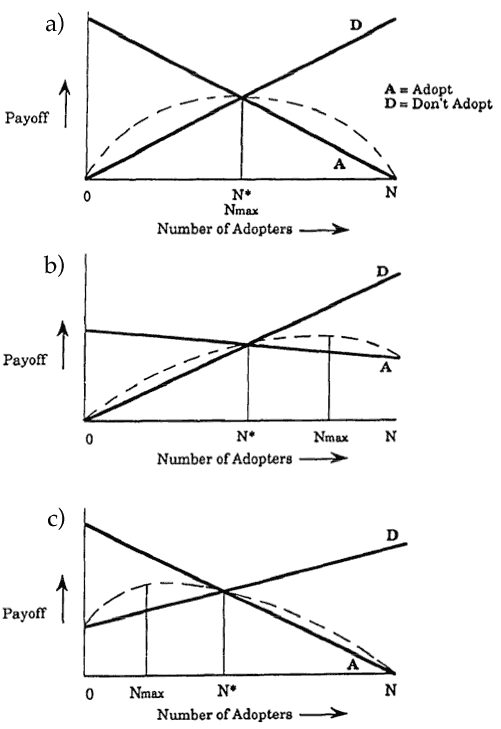
\includegraphics[width=1\linewidth]{gfx/markusCongestedTextProcessor}}
		\caption[>>Payoff<< durch Nutzung zweier Textverarbeitungsmaschinen \newline \citep{Markus:1990}]{Die Grafiken illustrieren drei Szenarios der Entwicklung des tatsächlichen Nutzen (>>Payoff<<) für die Abteilung durch Einführung eines zweiten Computers mit einem Textverarbeitungsprogramm.}\label{fig:markusText}
\end{figure}
	
	Der Abteilungsleiter entscheidet daher, einen zweiten Computer anzuschaffen und teilt dies der Belegschaft mit. In dieser Situation ist es wahrscheinlich, dass das Verhalten der Mitarbeiter den maximalen Nutzen der zweiten Maschine verhindert. Jeder hat zwei Optionen offen und kann entweder auf den neuen Computer umsteigen (\emph{A} für >>Adopt<<) oder beim alten bleiben (\emph{D} für >>Don't Adopt<<). \hyperref[fig:markusText]{Abbildung \ref*{fig:markusText}a} zeigt eine theoretische Verteilung des tatsächlichen Nutzen der Einführung des zweiten Computers. Auf der horizontalen Achse ist die Anzahl der Mitarbeiter dargestellt, die auf das neue Gerät wechseln. \emph{N} bezeichnet die Gesamtanzahl aller Mitarbeiter. Die Linien \emph{A} und \emph{D} sind linear invers zueinander und stellen die Auslastung der beiden Geräte dar. Diese ergibt sich aus der Anzahl der jeweiligen Nutzer. Die vertikale Achse zeigt den Nutzen für die gesamte Abteilung. Theoretisch erreicht man einen maximalen Nutzen für die Abteilung, wenn beide Geräte gleich ausgelastet sind, in der Praxis jedoch ist dies oft nicht der Fall.
	
	\medskip Es gibt viele Faktoren, die den Verlauf von \emph{A} und \emph{D} beeinflussen können, beispielsweise unterschiedliche Rechenleistungen und Performance der beiden Computer oder der Aufwand, der mit dem Erlernen eines neuen User Interface am neuen Rechner verbunden ist. \hyperref[fig:markusText]{Abbildung \ref*{fig:markusText}b} und \hyperref[fig:markusText]{Abbildung \ref*{fig:markusText}c} zeigen zwei weitere mögliche Szenarios, bei denen der maximale Nutzen dann erreicht wird, wenn der größere Teil der Belegschaft entweder beim alten Gerät bleibt oder zum neuen wechselt.
	
	Dieses Beispiel zeigt, dass es notwendig ist, spezielle Situationen genau zu analysieren und entsprechend darauf zu reagieren. So läge es hier am Abteilungsleiter, die optimale Auslastung der beiden Geräte zu finden und zu forcieren. Die gegenseitige Abhängigkeit, die in solch einem Szenario entsteht, ist der Grund für diese unterschiedlichen Ergebnisse \citep{Markus:1990}.
	
	\medskip Als zweites Beispiel behandeln Markus und Connolly ein System zur automatischen Planung von Meetings, genauso wie Jonathan Grudin in seiner Studie \citep{Grudin:1988p126}. Dieses System wird für eine Gruppe von Personen in einem Unternehmen eingeführt, die untereinander alle ungefähr gleich vielen Meetings beiwohnen. Damit sei gesichert, dass theoretisch jeder gleich viel vom System profitieren kann. 
	
	In diesem Szenario sind >>Adopter<< jene Personen, die regelmäßig ihre Termine in das System eintragen und pflegen. Sobald Termine eingetragen werden, sind sie für alle zugänglich. Daher haben >>Non-Adopter<< einen Vorteil: sie haben keinen zusätzlichen Aufwand, da sie nichts eintragen, trotzdem verfügen sie über alle Informationen im System. Diese Situation kann auch als >>multi-person prisoner's dilemma<< bezeichnet werden \citep{Schelling:1987}.

\begin{figure}
	{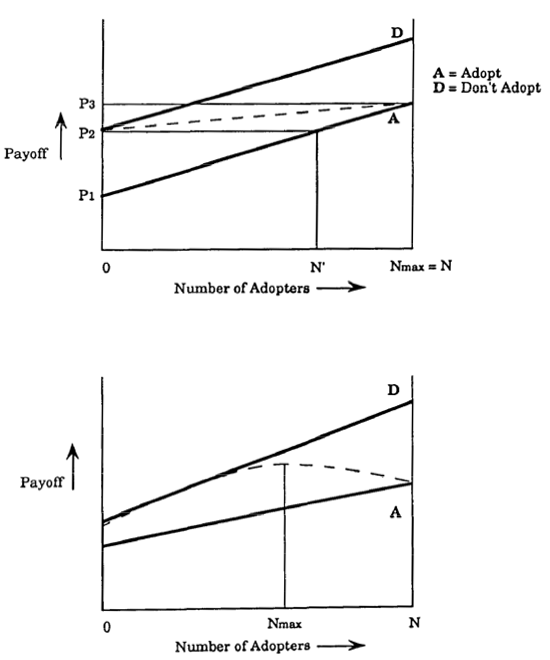
\includegraphics[width=1\linewidth]{gfx/markusMeetingPlanner}}
\caption[>>Payoff<< durch Nutzung eines automatischen Meeting Planers \newline \citep{Markus:1990}]{Die Grafiken illustrieren zwei Szenarios der Entwicklung des tatsächlichen Nutzen (>>Payoff<<) für die Abteilung durch Einführung eines automatischen Meeting Planers.}\label{fig:markusMeeting}
\end{figure}

In \hyperref[fig:markusMeeting]{Abbildung \ref*{fig:markusMeeting}a} wird der Nutzen von >>Adoptern<< und >>Non-Adoptern<< als zwei parallele Linien dargestellt. Die Differenz dieser beiden Werte bezeichnet den zusätzlichen Aufwand, den nur >>Adopter<< haben. Deswegen ist ihr Nutzen geringer. Man erkennt sofort, dass es irrelevant ist, wie viele Personen das System nutzen und wie viele nicht, denn diejenigen, die es nicht nutzen, werden immer einen Vorteil haben. Dies bedeutet aber auch, dass es für jeden das Beste wäre, das System nicht zu nutzen, weshalb es zu Schwierigkeiten bei der Einführung eines solchen Systems kommen könnte. In so einem Fall läge es wiederum am Abteilungsleiter, entsprechende Maßnahmen zu ergreifen, damit sich dieses ungleiche Verhältnis verbessert. 

\hyperref[fig:markusMeeting]{Abbildung \ref*{fig:markusMeeting}b} zeigt eine Situation, in der sich ausreichen Mitarbeiter zusammenschließen und gemeinsam in einer Koalition das System nutzen. Sie schaffen dadurch den selben kollektiven Nutzen für >>Adopter<<, wie wenn keiner das System verwenden würde. Dies setzt natürlich voraus, dass die Koalition über genügend Mitglieder verfügt, da die Rechnung sonst nicht aufgeht.

\medskip Im letzten Beispiel erläutern Markus und Connolly die Relevanz der kritischen Masse. Sie untersuchen dazu ein neu eingeführtes Kommunikationssystem, das es den Mitarbeitern erlaubt, intern mittels E-Mail zu kommunizieren. Vor Einführung dieses neuen Systems standen den Angestellten das Telefon, face-to-face Meetings und interne Post als Kommunikationsmittel zur Verfügung. 

Es ist offensichtlich, dass der Nutzen dieses neuen Mediums für die ersten >>Adopter<< relativ gering ist. Genauso wie das Telefon macht das E-Mail System wenig Sinn, wenn es nicht von jedem genutzt wird. Gibt es aber genügend Personen die es nutzen, steigt der Nutzen für alle stark an, unter Umständen sogar so weit, dass er den Nutzen anderer Kommunikationskanäle übersteigt. 

\medskip \hyperref[fig:markusMass]{Abbildung \ref*{fig:markusMass}a} zeigt den Punkt der kritischen Masse dort, wo die >>Payoff<< Linien von >>Adoptern<< und >>Non-Adoptern<< sich schneiden. Der tatsächliche Nutzen für das Kollektiv wird durch die gestrichelte Linie dargestellt. Für das einzelne Individuum ist es vor Erreichen der kritischen Masse vorteilhafter, nicht auf das neue System umzusteigen, doch nach Erreichen der kritischen Masse ist das Umsteigen vorteilhafter. Der steigende Nutzen vor der kritischen Masse für >>Non-Adopter<< ergibt sich aus der Annahme, dass durch mehr >>Adopter<< weniger Personen die alten Kommunikationsmittel nutzen und diese dadurch entlastet werden. >>Non-Adopter<< finden also leichter freie Räume für Meetings und kommen auf telefonischem Wege leichter zu anderen Mitarbeitern durch, da deren Linien seltener besetzt sind. In dieser Situation erreicht der Nutzen für das kollektiv seinen Höchststand, wenn alle Mitarbeiter das neu System verwenden. 

\medskip \hyperref[fig:markusMass]{Abbildung \ref*{fig:markusMass}b} stellt einen sinkenden Nutzen für >>Non-Adopter<< dar, während die Anzahl der >>Adopter<< steigt. Diese Situation könnte beispielsweise eintreten, wenn Personen wichtige Informationen nicht erhalten, nur weil sie das neue E-Mail System nicht nutzen. Höchst interessant ist in dieser Illustration die Tatsache, dass, wenn niemand das neue System verwendet, ein gleich hoher Nutzen für das Kollektiv entsteht, wie wenn alle es verwenden.

\begin{figure}
	{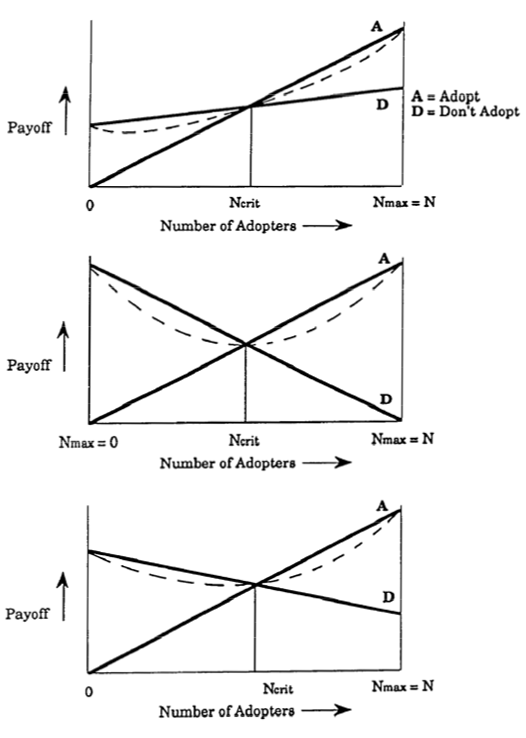
\includegraphics[width=1\linewidth]{gfx/markusCriticalMass}}
\caption[Die kritische Masse \newline \citep{Markus:1990}]{Die Grafiken illustrieren drei Szenarios der kritischen Masse unter verschiedenen Umständen.}\label{fig:markusMass}
\end{figure}

\medskip \hyperref[fig:markusMass]{Abbildung \ref*{fig:markusMass}c} geht von einem noch pessimistischeren Szenario aus und zeigt den maximalen Nutzen wenn jeder Mitarbeiter auf das neue System umsteigt. Wichtig ist hier jedoch die Tatsache, dass die Belegschaft besser dran ist, wenn keiner umsteigt, als wenn nur einige, sprich weniger Personen als für die kritische Masse notwendig, umsteigen. Das bedeutet, solange die Rate der Umsteiger sich nicht 100\% nähert, ist es vorteilhafter, wenn keiner der Mitarbeiter umsteigt.

\medskip Aus diesen designierten Szenarios wird ersichtlich, dass die gegenseitigen Abhängigkeiten, denen Groupware unterliegt, eng verknüpft sind mit Nutzen und Schaden, die das jeweilige System anrichten kann. Diese Eigenheiten müssen beim Design von Groupware beachtet werden, damit der Erfolg selbiger nicht gefährdet ist. \citep{Markus:1990}

\section*{Zusammenfassung}
In der Wissenschaft gibt es verschiedene Definitionen und Auslegungen des Begriffes >>Computer Supported Cooperative Work<<. Die Wurzel dieser Uneinigkeit findet sich schon tiefer, bei der genauen Definition und Unterscheidung von >>Collaborative Work<<, >>Collective Work<< und >>Cooperative Work<<. Viele Wissenschaftler verwenden die Begriffe synonym, andere hingegen bestehen auf einer klaren Trennung der Termini. Für die Zwecke dieser Arbeit reicht jedoch eine synonyme Verwendung aus, denn letztendlich bezeichnet der Begriff \ac{CSCW} ein multidisziplinäres Forschungsgebiet, das kooperative Zusammenarbeit innerhalb Gruppen untersucht und Technologien zur Förderung und Unterstützung selbiger entwickelt. Unter >>Groupware<< versteht man alle Systeme, egal ob Hard- oder Software, welche die in \ac{CSCW} gewonnenen Erkenntnisse in die Praxis, zum Zwecke der Verbesserung von Teamwork, umsetzen. Design und Entwicklung solcher Systeme ist eine schwierige Aufgabe und wird von vielen verschiedenen Faktoren beeinflusst, die über Erfolg oder Misserfolg entscheiden. Es gibt Frameworks und Patterns, die versuchen formale Richtlinien zu geben, jedoch bildet jedes System und vor allem das Umfeld, in dem es eingesetzt wird, einen einzigartigen Kontext, der genau analysiert und berücksichtigt werden muss.

